\documentclass[compress,8pt]{beamer}
\usetheme{bredele}
%\documentclass[handout,8pt]{beamer} % pour passer
%\usepackage{pgfpages} % En A4, il faut
%\pgfpagesuselayout{resize to}[a4paper,border shrink=5mm,landscape] %Ajouter ces trois lignes
%\usepackage{beamerthemeshadow}



%%%%%%%%%%%%%%%%%%%%%%%%%%%%%%%%%%%%%%%%%%%%%%%%



\title[Titre version courte]{Placez votre titre ici dans sa version longue}
% Titre du diaporama

\subtitle{Vous pouvez ajouter un sous-titre}
% Sous-titre optionnel

\author{Marcel Dupont\inst{1}}
% La commande \inst{...} Permet d'afficher l' affiliation de l'intervenant.
% Si il y a plusieurs intervenants: Marcel Dupont\inst{1}, Roger Durand\inst{2}
% Il suffit alors d'ajouter un autre institut sur le modèle ci-dessous.

\institute[Université de Knackenheim]
{
  \inst{1}%
  Molécules et fluides intermittents\\
  Institut de la Grande Gudule
  }


\date{18 Brumaire 2015}
% Optionnel. La date, généralement celle du jour de la conférence

\subject{Sujet de votre diaporama}
% C'est utilisé dans les métadonnes du PDF



\logo{

\includegraphics[scale=0.15]{images/logo.png}
}



%%%%%%%%%%%%%%%%%%%%%%%%%%%%%%%%%%%%%%%%%%%%%%%%%%%%%%%%%%%%%%%%%%%%%
\begin{document}

\begin{frame}
  \titlepage
\end{frame}





\begin{frame}{Sommaire}
  \tableofcontents
  % You might wish to add the option [pausesections]
\end{frame}

% Section and subsections will appear in the presentation overview
% and table of contents.

\section{Les blocs}

\begin{frame}{Les blocs}

\begin{block}{Bloc simple}
\begin{itemize}
\item Premier point
\item Second point
\item Troisième point
\end{itemize}
\end{block}

\begin{exampleblock}{Bloc exemple}
\begin{itemize}
\item Premier point
\item Second point
\item Troisième point
\end{itemize}
\end{exampleblock}

\begin{alertblock}{Bloc alert}
\begin{itemize}
\item Premier point
\item Second point
\item Troisième point
\end{itemize}
\end{alertblock}
\end{frame}


\section{Les bo\^ites}

\begin{frame}{Les boites}

\begin{columns}

\begin{column}{0.5\textwidth}
\boitejaune{
Ceci est \\
une boite jaune
}

\boiteorange{
Ceci est \\
une boite orange
}

\boitemarron{
Ceci est \\
une boite marron
}
\end{column}

\begin{column}{0.5\textwidth}
\boiteviolette{
Ceci est \\
une boite violette
}

\boitebleue{
Ceci est \\
une boite bleue
}

\boitegrise{
Ceci est \\
une boite grise
}

\end{column}

\end{columns}


\end{frame}



\section{Les listes}
	\subsection{Liste à item}

\begin{frame}{Titre de la frame}

	\begin{itemize}
		\item premier élément de liste,
		\item deuxième élément de liste,
		\item troisième élément de liste.
	\end{itemize}
\end{frame} 

		\subsection{Liste énumérative} 
\begin{frame}{Titre de la frame} 
	\begin{enumerate}
		\item élément de liste numéro 1,
		\item élément de liste numéro 2,
		\item élément de liste numéro 3.  
	\end{enumerate}
\end{frame}


		\subsection{Liste descriptive} 
\begin{frame}{Titre de la frame} 
	\begin{description}
		\item [Thème de présentation : ] ces thèmes sont en fait...
		\item [Thème de couleur : ] gère tout ce qui est couleur...
		\item [Thème de police : ] s'occupe de tout ce qui est police, gras...
		\item [Thème interne : ] s'occupe de l'apparence des éléments...
	\end{description}
\end{frame}



\section{Le texte}

\begin{frame}{Titre de la frame} 

Voici du texte normal

\alert{Voici du texte \texttt{alert}}

\exemple{Voici du texte \texttt{exemple}}

\emph{Voici du texte \texttt{emphase}}

\end{frame}



\section{Les images}

\begin{frame}{Titre de la frame} 

\begin{figure}
\centering
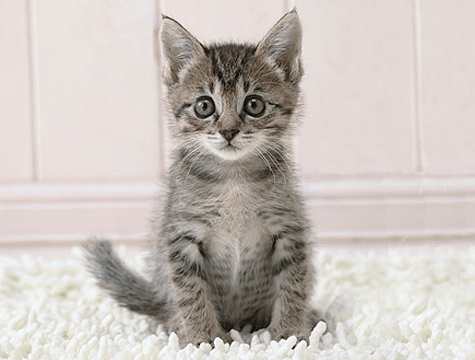
\includegraphics[scale=0.3]{images/chaton.png}
\caption{Ceci est un poisson}
\end{figure}

\end{frame}



\end{document}


